\section{Модификация проекта «Изображение проекции полиэдра»}

\subsection{Постановка задачи}

Все рёбра делятся на три класса: \emph{полностью видимые}, \emph{видимые частично} и \emph{полностью невидимые}. Назовём грань «гранью с полностью видимыми рёбрами», если все образующие её рёбра полностью видимы. Если все образующие грань рёбра полностью невидимы, то грань будем называть «гранью с полностью невидимыми рёбрами». Все остальные грани будем называть «гранями с частично видимыми рёбрами». Модифицируйте эталонный проект таким образом, чтобы определялась и печаталась следующая характеристика полиэдра: \emph{сумма периметров проекций «граней с частично видимыми рёбрами», проекция центра которых находится строго вне квадрата единичной площади с центром в начале координат и сторонами, параллельными координатным осям}.
~(28).

\subsection{Теоретические аспекты}

Задача изображения проекции полиэдра без невидимых рёбер может быть решена следующим образом: будем отображать отрезки~--- проекции рёбер полиэдра, причём части рёбер, \emph{затенённые} гранями полиэдра, учитывать не нужно.
Полиэдр задаётся тремя наборами: вершин, рёбер, граней, соответствием между ними и вращением трёхмерного пространства. Проектирование производится при помощи бесконечной перспективы~(Физическая интерпретация: свет падает на объект из бесконечно удалённой точки параллельным потоком и мы видим тень объекта на плоскости, перпендикулярной вектору направления света). Далее вектор направления света будем называть \emph{вектором проектирования}.

Механизм проектирования предельно прост: после преобразования координат~(пространственный поворот на соответствующие углы Эйлера и гомотетия) для отображения точки достаточно лишь \emph{забыть} её $z$-координату.

Вкратце опишем алгоритм \emph{затенения} ребра гранью:
Рассмотрим произвольное ребро. Каждая грань разбивает его на \emph{затенённые} и \emph{освещённые} участки. Несложно показать что в нашем случае~(грани-выпуклые многоугольники) освещённая часть представляет собой либо ребро, либо $\O$.~(см. рис.\ref{fig:poly_shadow})

\begin{figure}[ht!]
\begin{center}
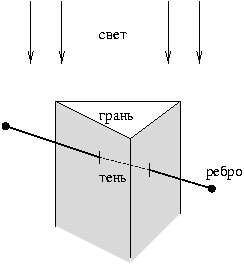
\includegraphics[scale=1]{images/pol_shad.png}
\caption{Затенение ребра гранью} \label{fig:poly_shadow}
\end{center}
\end{figure}

Для получения конечного результата необходимо учесть тени от всех граней~(Утверждение открывает широкий простор для оптимизации~--- нахождения достаточного условия). 

Воспользовавшись тем фактом что ребро~--- одномерный объект, задачу нахождения пересечения освещённых областей от всех граней можно свести к задаче поиска дополнения покрытия интервала $(0,1)$ набором других интервалов. Тень от грани~--- пересечение ребра и открытой бесконечной призмы, сверху ограниченной гранью, а с <<боков>>~--- плоскостями, содержащими рёбра грани и вектор проектирования, нормали которых направлены внутрь призмы. Процесс построения призмы показан на рисунке \ref{fig:poly_prism}.

\begin{figure}[ht!]
\begin{center}
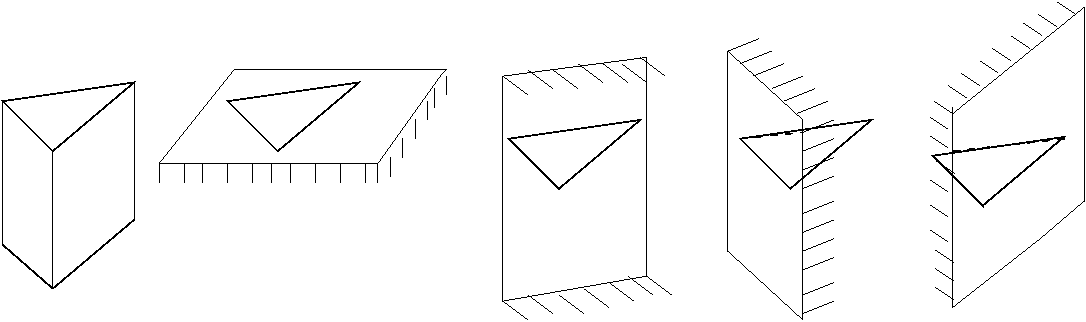
\includegraphics[scale=0.6]{images/pol_prism.png}
\caption{Построение призмы затенения} \label{fig:poly_prism}
\end{center}
\end{figure}

\subsection{Детали реализации}

Таким образом мы можем сказать какие рёбра будут \emph{видимыми}, а какие \emph{невидимыми}, что соответственно позволяет нам определить какие гани являются \emph{частично видимыми}.

Метод грани, решающий эту задачу:
\begin{lstlisting}
class Facet
    
    ...

  def part_vis?
    return false if !@edges
    pr1,pr2 = true, true
    trtab = @edges.map{|edge| [edge.compl_visible?,edge.invisible?]}
    trtab.each{|x|pr1&&=x[0];pr2&&=x[1]}
    !(pr1||pr2)
  end 
end
\end{lstlisting}

Естественно для этого требуется знать какие рёбра принадлежат грани. Воспользуемся структурой данных <<хэш>> для удаления дубликатов рёбер и затем поставим каждой грани в соответствие набор рёбер, ей принадлежащих. Это можно сделать при помощи простой проверки что множество вершин грани содержит концы ребра.
\begin{lstlisting}
  def edges_uniq
    edges = {}
    @edges.each do |e|
      if edges[[e.beg, e.fin]].nil? && edges[[e.fin, e.beg]].nil?
        edges[[e.beg, e.fin]] = e
      end
    end
    @edges = edges.values
  end
\end{lstlisting}

Наконец, для определения положения центра грани необходимо проверить что его координаты  в изначальной системе отсчёта соответствуют неравенствам:
$|x_c|>0,5$ и $|y_c|>0,5$. Откуда следует что параметры проектирования должны быть известны в классе \verb|Polyedr|. 
Код метода, решающего эту задачу:
\begin{lstlisting}
  def outside_sqr?(alpha,beta,gamma,c)
    cent = center
    cent = cent.rz(-gamma).ry(-beta).rz(-alpha)*(1/c)
    (cent.x>0.5||cent.x<-0.5)&&(cent.y>0.5||cent.y<-0.5)
  end
\end{lstlisting}

В итоге все методы, требующиеся для решения поставленной задачи описаны и остаётся только проверить все грани на соответствие условиям задачи и сложить периметры граней им удовлетворяющих.
На рисунке \ref{fig:poly_fig} представлен результат работы программы, где точками отмечены центры граней, удовлетворяющих условиям задачи.

\subsection{Возможные обобщения}
Задачу можно обобщить, например, потребовав покрывать грани какой-либо текстурой и описывать условия задачи с учётом текстуры. Другой задачей может быть поиск суммы расстояний между правильными пирамидами. построенными на гранях полиэдра, как на основаниях.

\begin{figure}[ht!]
\begin{center}
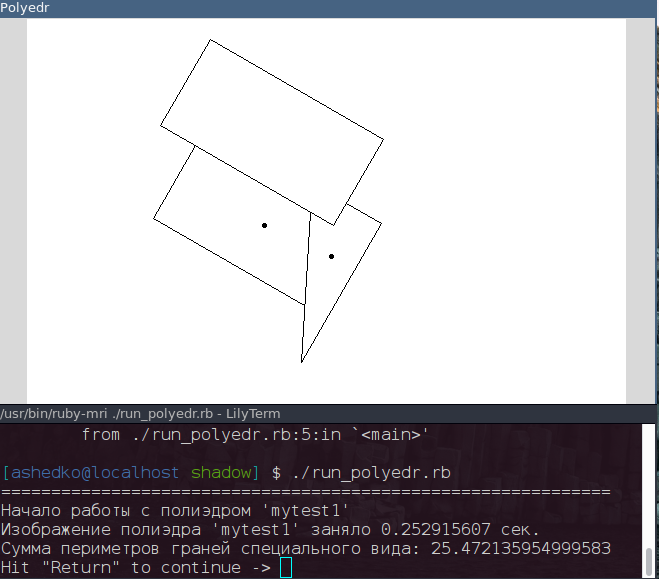
\includegraphics[scale=0.8]{images/poly_1.png}
\caption{Иллюстрация работы программы} \label{fig:poly_fig}
\end{center}
\end{figure}